\section{Durchführung}
Zu Beginn soll die Zeitabhängigkeit der Schwingungsamplitude untersucht werden, dafür
wird der kleinere der beiden in der Schaltung "verfügbaren" Widerstände verwendet.
Eine Darstellung der verwendeten Schaltung ist in Abbildung \ref{fig:a} zu sehen.
\begin{figure}[H]
  \centering
  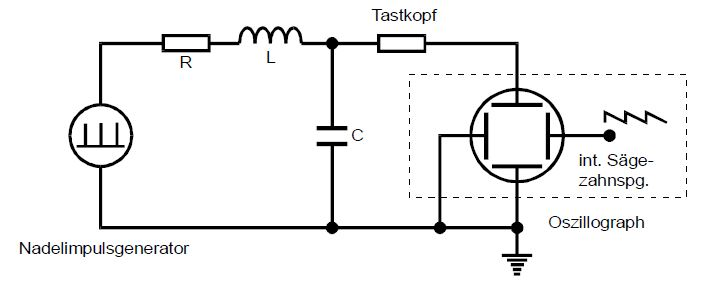
\includegraphics[width=13cm]{a.JPG}
  \caption{Schaltung zur Untersuchung der Zeitabhängigkeit der Ampitude}
  \cite{skript}.
  \label{fig:a}
\end{figure}
Der Schwingkreis wird mit einem Nadelimpuls angeregt. Es ist darauf zu achten, dass
eine erneute Anregung erst erfolgt, wenn die Amplitude der gedämpften
Schwingung um den Faktor 3 bis 8 abgeklungen ist. Auf dem Oszilloskop lässt
sich nun der Verlauf der Schwingungskurve verfolgen und es wird ein
Thermodruck angefertigt.
Der Eingangswiderstand des Oszilloskops kann hir vernachlässigt werden, da der
Tastknopf einen sehr hohen Innenwiderstand ($R_{i}=\SI{10}{\mega\ohm}$) besitzt.

Im Folgenden soll der Widerstand $R_{ap}$ bestimmt werden, ab dem der apperiodische
Grenzfall eintritt. Dazu wird die Schaltung aus Abbildung \ref{fig:b} verwendet.
\begin{figure}[H]
  \centering
  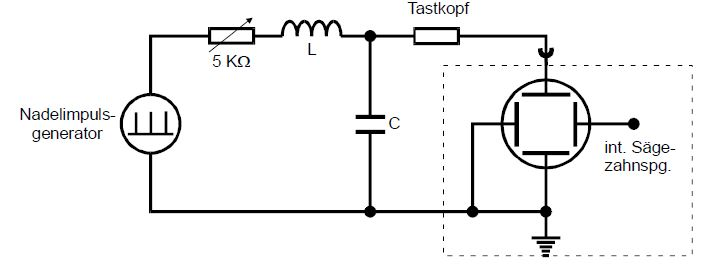
\includegraphics[width=13cm]{b.JPG}
  \caption{Schaltung zur bestimmung des aperiodischen Grenzwiderstandes $R_{ap}$}
  \cite{skript}.
  \label{fig:b}
\end{figure}
An dem regelbaren Widerstand wird zunächst ein Maximaler Widerstand eingestellt.





\label{sec:Durchführung}
